\chapter{Переход Фредерикса и изменение равновесной ориентационной структуры ХЖК во внешнем электрическом поле.}\label{ch:ch2}
\section{Система уравнений Эйлера-Лагранжа и упрощение функционала свободной энергии}\label{sec:ch2/sec1}
Первая вариация свободной энергии~\eqref{eq:free-energy} может быть записана следующим образом:
\begin{multline}
\delta \FF_\mathrm{tot} = S_{\!\bot} \left\{\int_0^L \left[ {\frac12\frac{d\AA}{d\theta}\, \theta'^2 \delta\theta + \AA\theta' \delta\theta'} + \frac12\frac{d B}{d\theta}\,\phi'^2\delta\theta\right. + \right.\\
\left.+ B \phi' \delta \phi'- \frac{d C}{d\theta}\,\phi'\delta\theta - C\delta\phi'\right]\, dz + \\
{+\frac12\!\sum_{\alpha=1,2}\left(W_\theta^{(\alpha)}\!\sin2(\theta_\alpha- \theta_0^{(\alpha)})\delta\theta_\alpha + W_\phi^{(\alpha)}\!\sin2(\phi_\alpha - \phi_0^{(\alpha)})\delta\phi_\alpha\right)} + \\
\left. {+\frac{\varepsilon_a}{8\pi} \EuScript{U}^2J^2\int_0^L \frac{\sin 2\theta }{\EE^{2}(\theta)}\delta\theta\, dz
	+\left.\bar{e}\EuScript{U} J \frac{\sin 2\theta }{\EE(\theta)}\delta\theta\right|^L_0
}\right\}.
\label{deltaF_tot}
\end{multline}
Проинтегрировав по частям вклады в $\delta\FF_\mathrm{tot}$, содержащие вариации производных и приравнивая к нулю $\delta \FF_\mathrm{tot}$ для произвольных вариаций $\delta\theta$ и $\delta\phi$ в объёме и на границах, получаем систему из двух уравнений Эйлера-Лагранжа 
\begin{eqnarray}
&&\frac{d\AA}{d\theta}\theta'^2 + 2\AA \theta'' = \frac{d B}{d\theta}\phi'^2 - 2\frac{d C}{d\theta}\phi'
+ \frac{\varepsilon_a\EuScript{U}^2\! J ^2\!\sin 2\theta}{4\pi\EE^2(\theta)} ,
\label{eq:E-L1}\\
&&{d}\left( B\phi' - C \right)/{dz} = 0,
\label{eq:E-L2}
\end{eqnarray}
и двух граничных условий
\begin{eqnarray}
&&\left(2(-1)^\alpha [{\AA(\theta)\theta'} + \bar{e} {\EuScript{U}}J\sin2\theta/\EE(\theta)]\phantom{ W_\phi^{(\alpha)}}\right. + \nonumber\\
&&\hspace{27mm}\left.\left.+ W_\theta^{(\alpha)}\sin2(\theta - \theta_0^{(\alpha)})\right) \right|_{z=l_\alpha} = 0,\label{eq:gran-1}\\
&&{\left.\left(2(-1)^\alpha (B\phi' - C)
	+W_\phi^{(\alpha)}\sin2(\phi - \phi_0^{(\alpha)})\right) \right|_{z=l_\alpha}} = 0,
\label{eq:gran-2}
\end{eqnarray}
где $\alpha = 1, 2$.
Из уравнений~\eqref{eq:E-L1} и~\eqref{eq:E-L2} можно сделать вывод, что функция $\theta(z)\in C^2[0,\, L]$, а $\phi(z)\in C^1[0,\, L]$.
Заметим, что~\eqref{eq:E-L1} -- функциональное интегро-дифференциальное уравнение, так как $J_1$ зависит от значений $\theta(z)$ на границах, а $J$ содержит интеграл~\eqref{eqD_z}.
Кроме того, граничные условия~\eqref{eq:gran-1} являются нелокальными.
Данные свойства, как уравнения, так и граничных условий, возникли благодаря учёту флексоэлектрической поляризации.

Первый интеграл системы уравнений~\eqref{eq:E-L1} и~\eqref{eq:E-L2} выглядит следующим образом:
\begin{eqnarray}
&&{\AA(\theta)\theta'^2}+  B(\theta)\varphi'^2 {-\EuScript{U}^2 J ^2/(4\pi\EE(\theta))} =C_1,
\label{eq:theta'}\\
&&B(\theta)\phi' -C(\theta)= C_2,
\label{eq:phi'}
\end{eqnarray}
где $C_{1,2}$ -- произвольные константы.
Конкретные значения этих констант могут быть найдены из граничных условий~\eqref{eq:gran-1} и~\eqref{eq:gran-2}.

Ввиду сложности возникающих уравнений Эйлера-Лагранжа удобно искать равновесную ориентационную структуру ХЖК, используя прямые методы минимизации свободной энергии.
При этом уравнение~\eqref{eq:phi'} и граничные условия~\eqref{eq:gran-2} позволяют упростить выражение для полной свободной энергии $\FF_\mathrm{tot}$, а уравнение~\eqref{eq:theta'} и граничные условия~\eqref{eq:gran-1} дают возможность контролировать точность результатов численных расчётов.
В решении задачи поиска равновесных профилей углов оказывается возможным записать $\FF_\mathrm{tot}$ как функционал, зависящий только от $\theta(z)$.
Для этого используем выражение для $\phi'$, полученное из соответствующего уравнения Эйлера-Лагранжа.
Таким образом, мы будем рассматривать $\FF_\mathrm{tot}[\theta(z)]$, содержащий равновесное распределение $\phi(z)$, подстраивающееся под заданное распределение $\theta(z)$.
%Ограничиваясь только равновесными профилями углов $\theta(z)$ и $\phi(z)$, можно записать $\FF_\mathrm{tot}$ как функционал, зависящий только от $\theta(z)$.

Рассмотрим выражение~\eqref{eq:F_e_basic} для свободной энергии, связанной с объёмной ориентационной упругостью ХЖК.
Подставив в него $\phi'$, выраженное из~\eqref{eq:phi'}, получим
\begin{equation}
\FF_\mathrm{e} = \FF^{(0)}_\mathrm{e} + \frac{S_{\!\bot}}{2}\int_0^L \left[ A(\theta) \theta'^2 + \frac{C_2^2 - C^2(\theta)}{B(\theta)} \right]\, dz.
\label{eq:F_e_2}
\end{equation}
В выражение~\eqref{eq:F_e_2} входит константа $C_2$.
Для того, чтобы определить её, проинтегрируем $\phi'$ из~\eqref{eq:phi'} по отрезку $[0,L]$:
\begin{equation}
\phi_\mathrm{tot} = C_2 I_1 + I_2,
\label{eq:help_find_C1-2}
\end{equation}
где $\phi_\mathrm{tot}  =  \phi(L) - \phi(0)$,
$$
I_1 = \int_0^L \frac{dz}{B(\theta)}, \;
I_2  =  \int_0^L \frac{C(\theta)}{B(\theta)}\, dz.
$$
Подставляя~\eqref{eq:phi'} в~\eqref{eq:gran-2}, получаем
\begin{equation}
{2\left(\phi(l_\alpha)-\phi_0^{(\alpha)}\right)=(-1)^{\alpha+1}\arcsin\left(2C_2/W_\phi^{(\alpha)}\right)},
\label{eq:help_find_C1-0}
\end{equation}
$\alpha=1,2$, следовательно,
\begin{equation}
\!\!{2(\phi_\mathrm{tot}^{(0)}-\phi_\mathrm{tot})
	=\arcsin({2C_2}/{W_{\phi}^{(1)}})+\arcsin({2C_2}/{W_{\phi}^{(2)}})},
\label{eq:help_find_C1}
\end{equation}
где $\phi_\mathrm{tot}^{(0)}=\phi_0^{(2)}-\phi_0^{(1)}$.
Здесь предполагается, что $\left|\phi(l_\alpha)-\phi_0^{(\alpha)}\right|\leq \pi/4$.
Это ограничение соответствует отсутствию скачкообразных изменений шага спирали ХЖК~\autocite{BelyakovJumpsPhysRevE2005}.

Из~\eqref{eq:help_find_C1-2} и \eqref{eq:help_find_C1} можно выразить константу $C_2$,
\begin{equation}\label{eq:C2iteration}
C_2=(\varphi_\textrm{tot}^{(0)}-I_2)/\big(I_1+k_1/W^{(1)}_\varphi + k_2/W^{(2)}_\varphi \big),
\end{equation}
где $k_\alpha=\left(W^{(\alpha)}_\varphi/2C_2\right)\arcsin\left(2C_2/W^{(\alpha)}_\varphi \right)$, $1\leq k_\alpha\leq \pi/2$.
Неравенства $\left|C_2\right|/W^{(\alpha)}_\varphi \leq 0.5$ должны выполняться, чтобы существовало решение трансцендентного уравнения~\eqref{eq:C2iteration}.
Для случая $\left|C_2\right|/W^{(\alpha)}_\varphi \ll 1$ можно записать точное выражение для $C_2$:
\begin{equation}\label{eq:C2implicit}
{C_2=(\varphi_\textrm{tot}^{(0)}-I_2)\left(I_1+{2}/{W_\phi^{H}}\right)^{-1}}
\end{equation}
где $W_\phi^{H} = {2W_\phi^{(1)}W_\phi^{(2)}}/(W_\phi^{(1)} + W_\phi^{(2)})$.


Подставляя выражение~\eqref{eq:C2iteration} в~\eqref{eq:F_e_2} и используя~\eqref{eq:help_find_C1-0}, получаем следующее выражение для полной свободной энергии $\FF_\mathrm{tot}$ как функционала, зависящего только от $\theta(z)$:
\begin{multline}
\FF_\mathrm{tot}(\theta) = \FF^{(0)}_e + \frac{S_{\!\bot}}{2}\Bigg[\int_0^L \left({ \AA(\theta)}\theta'^2 - \frac{C^2(\theta)}{B(\theta)} \right) dz +\\
+W_\theta^{(1)}\sin^2 \left( \theta(0) - \theta_0^{(1)} \right)+W_\theta^{(2)}\sin^2 \left( \theta(L) - \theta_0^{(2)} \right) +\\
+
C_2^2\left(I_1+{\kappa_1}/{W^{(1)}_\varphi}+{\kappa_2}/{W^{(2)}_\varphi}\right)-{\frac{\EuScript{U}^2 J}{4\pi} }\Bigg],
\label{eq:F_for_minimization}
\end{multline}
где $\kappa_\alpha=2/\Big(1+\sqrt{1-\big(2C_2/W^{(\alpha)}_\varphi\big)^2}\Big)$, $1\leq \kappa_\alpha\leq 2$.
При $\left|C_2\right|/W^{(\alpha)}_\varphi \ll 1$ предпоследнее слагаемое в~\eqref{eq:F_for_minimization} может быть приближённо записано как
\begin{equation}\label{LastTermFtot_theta_implicit}
\frac{S_{\!\bot}}{2}\left( \phi_\mathrm{tot}^{(0)} - I_2 \right)^2\left(I_1+{2}/{W_\phi^{H}}\right)^{-1}.
\end{equation}
Погрешность такой аппроксимации составляет около 2\% при $\left|C_2\right|/W^{(\alpha)}_\varphi \leq 0.25$ и около 15\% для всей области $\left|C_2\right|/W^{(\alpha)}_\varphi\leq 1/2$.

После нахождения равновесной функции $\theta(z)$ можно найти соответствующую равновесную функцию $\phi(z)$, совмещая выражения~\eqref{eq:phi'}, \eqref{eq:gran-2} и~\eqref{eq:C2iteration}:
\begin{equation}\label{eq:phi_profile}
\varphi(z)=\varphi_0^{(1)}+\frac12\arcsin\frac{2C_2}{W^{(1)}_\varphi}
+ \int_0^z \frac{C(\theta)+C_2}{B(\theta)}\, dz .
\end{equation}

\section{Численная минимизация функционала свободной энергии}
Равновесную ориентационную структуру в ячейке ХЖК будем искать с помощью численной минимизации свободной энергии~\eqref{eq:F_for_minimization}, используя следующие углы лёгкого ориентирования на границах:
\begin{equation}\label{eq:initial}
\theta_0^{(1)}=\theta_0^{(2)}={\pi}/{2},\;\phi_\mathrm{tot}^{(0)}=q_0L.
\end{equation}
Эти условия соответствуют ненапряжённому ХЖК в отсутствие внешнего электрического поля.
Сведём задачу поиска минимума функционала $\FF_\mathrm{tot}[\theta(z)]$ к задаче поиска минимума функции нескольких переменных, аппроксимировав искомую зависимость $\theta(z)$ пробной функцией
\begin{equation}\label{eq:psi+Fourier}
\theta(z) =
\pi/2 + {\delta\psi}(z,\delta_1,\delta_2) + \sum\limits_{n=1}^N c_n\sin(\pi nz/L).
\end{equation}
Здесь слагаемое $\pi/2$ соответствует неискажённому состоянию.
Функция $\delta\psi(z,\delta_1,\delta_2)$, задаваемая выражением~\eqref{psi=}, содержит $\delta_1$ и $\delta_2$ -- отклонения от углов лёгкого ориентирования на границах: $\theta(0) = \pi/2 + \delta_1$, $\theta(L) = \pi/2 + \delta_2$.
Наконец, ряд Фурье описывает объёмные искажения ориентационной структуры, не затрагивающие границы.
Используя граничные условия~\eqref{eq:gran-1}, можно выразить коэффициенты $c_N$ и $c_{N-1}$ через все остальные -- $\delta_{1,2}$ и $\{c_n\}_{n=1}^{N-2}$.
Таким образом, углы $\delta_1$, $\delta_2$, а также коэффициенты $c_n$, $n=1,\dots,N-2$ являются регулируемыми параметрами.

Ограничимся в~\eqref{eq:psi+Fourier} $N = 20$ членами ряда Фурье.
Учёт более, чем 20 слагаемых приводит к относительному изменению профиля $\theta$ менее чем на $0.5\%$ для любого $z$ на всём интервале $[0,\, L]$.
В многомерной численной минимизации существует проблема попадания в максимумы или в седловые точки.
Для того, чтобы определить, действительно ли минимизация свободной энергии привела к минимуму, используем случайные небольшие сдвиги параметров  $\delta_{1,2}$, $\{c_n\}$ относительно полученных значений.
Если минимизационный алгоритм приводит к другому ответу, это означает, что предыдущий результат был ошибочным -- максимумом или седловой точкой.
При этом в случае, если достигнут, по крайней мере, локальный минимум, то при любом достаточно небольшом сдвиге минимизация будет всегда возвращать нас обратно.

Будем изменять напряжение $U$, зафиксировав все остальные параметры ячейки ЖК.
\begin{figure}
	\centering
	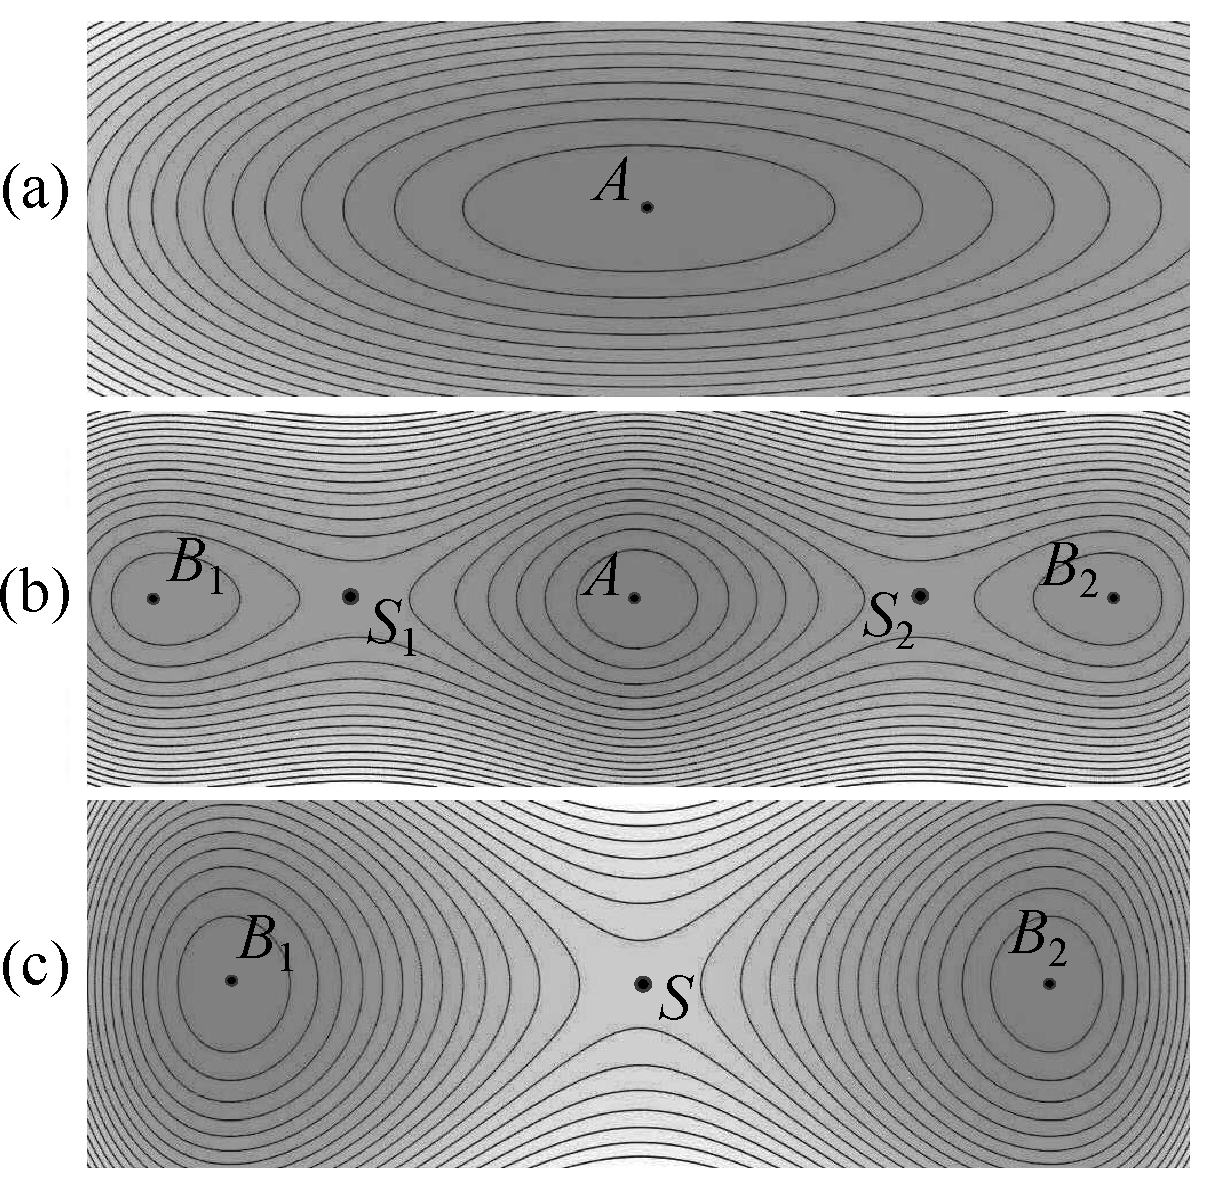
\includegraphics[width = 15cm]{Geo_final.eps}
	\caption{Схематичное двумерное изображение случаев, возникающих при численной минимизации свободной энергии}
	\label{pic_Geo_final}
\end{figure}
При этом будет наблюдаться один из трёх случаев, проиллюстрированных на Рис.~\ref{pic_Geo_final}:
\begin{enumerate}
	\item[(a)]
	Существует единственный минимум (точка А на рис.~\ref{pic_Geo_final}a), соответствующий планарной геликоидальной структуре, при этом $\delta_{1,2}=0$, $c_n = 0$, то есть $\theta(z)=\pi/2$, а $\phi(z) = q_0z$.
	\item[(b)]
	Случай трёх минимумов.
	Один из них (точка А на Рис.~\ref{pic_Geo_final}b) по-прежнему соответствует планарной геликоидальной структуре.
	Два других (точки $B_1$ и $B_2$) соответствуют искажённым структурам, то есть таким, для которых некоторые из параметров $\delta_{1,2}$, $c_n$ ненулевые.
	При этом параметры $(\delta_{1},\delta_{2},c_n)$, соответствующие точкам $B_1$ и $B_2$, отличаюся только знаком, следовательно, этим двум точкам соответствуют одинаковые распределения директора ввиду симметрии относительно замены ${\bf n} \leftrightarrow -{\bf n}$.
	\item[(c)]
	Имеются ровно два минимума.
	В этом случае существуют два минимума $B_1$ и $B_2$, соответствующие одной и той же искажённой ориентационной структуре.
	Планарная геликоидальная структура здесь не существует, так как является седловой точкой ($S$ на Рис.~\ref{pic_Geo_final}c).
\end{enumerate}
Здесь и далее мы будем называть ''устойчивыми'' равновесные состояния, соответствующие локальным минимумам свободной энергии, а ''метастабильными'' -- устойчивые состояния с энергией, большей, чем у другого устойчивого состояния.

\subsubsection{"Фазовая" \todo{(Структурная?)} диаграмма}

Случай (a) на Рис.~\ref{pic_Geo_final} возникает для напряжений $|U|$ ниже порогового значения $U^{**}$, а при достижении этого значения могут наблюдаться две различные ситуации.
Они соответствуют разрывному (I) и непрерывному (II) переходу Фредерикса:
\begin{itemize}
	\item[I.]
	В этом случае существует ещё одно пороговое значение $U^{*} > U^{**}$, при этом для $|U|\in (U^{**},\, U^{*})$ у функционала свободной энергииесть сразу три локальных минимума, из которых один соответствует начальной планарной геликоидальной структуре	, а два других -- искажённой ориентационной структуре, как показано на Рис.\ref{pic_Geo_final}b.
	Здесь $U^{**}$ -- наименьшее напряжение, при котором искажённая ориентационная структура ещё может существовать в качестве метастабильной, а, в свою очередь, $U^{*}$ -- максимальное напряжение, при котором планарная геликоидальная структура ещё может существовать как метастабильная.
	Таким образом, при любом $U$ из интервала $(U^{**},\,U^*)$ только одна из структур будет стабильной (с меньшей энергией), в то время как другая будет метастабильной.
	С ростом напряжения $|U|$ свободная энергия искажённой структуры уменьшается, и при $|U| = U_c$ становится равной энергии неискажённого состояния, и происходит разрывный переход Фредерикса.
	То есть, при $|U| < U_c$ более энергетически выгодным является неискажённое состояние, а при $|U| > U_c$ -- искажённое.
	Наконец, при $|U|>U^*$ реализуется случай (c).
	\item[II.]
	В данном сценарии существует только одно пороговое напряжение, $|U| = U_c$. Этот сценарий соответствует (I) для $U^{*} = U_c = U^{**}$, при этом происходит непрерывный переход Фредерикса. 
	Здесь при $|U| < U_c$ возникает случай (a), а при  $|U|>U_c$ -- случай (c), показанные на Рис.~\ref{pic_Geo_final}c.
\end{itemize}
Интервалы стабильности и метастабильности схематично изображены на Рис.~\ref{pic-U*U**Uc_otline}.
\begin{figure}%[thb]
	\centering
	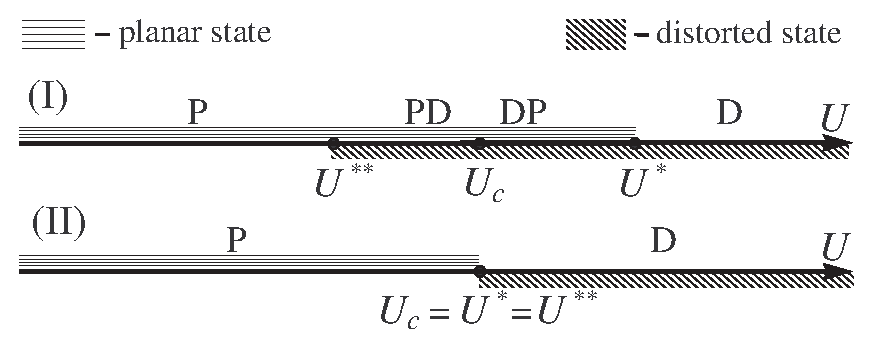
\includegraphics[width=12cm]{UU1d3a.eps}
	\caption{Иллюстрация разрывного (I) и непрерывного (II) переходов Фредерикса для $U > 0$.
		(I): Области устойчивости искажённой (D) структуры, $U>U^{**}$, и неискажённой (P) структуры, $U<U^{*}$.
		На интервале, обозначенном PD, $U^{**}<U<U_c$, искажённая структура метастабильна, а на интервале DP, $U_c < U < U^{*}$, метастабильна планарная геликоидальная структура.
		(II):  Области устойчивости для искажённой, $U > U_c$, и неискажённой структуры, $U < U_c$.}
	\label{pic-U*U**Uc_otline}
\end{figure}

Для того, чтобы изучить, как влияет флексоэлектрическая поляризация на переход Фредерикса, были рассчитаны пороговые напряжения $U^{**}$, $U_c$, $U^{*}$ для различных значений усреднённого флексоэлектрического коэффициента $\bar{e}$.
Отметим, что учёт флексоэлектричества привёл к тому, что значения напряжений $U^{**}$, $U^*$ и $U_c$ стали различными для  $U>0$ и $U<0$, если константы сцепления с подложкой различны, $W_\theta^{(1)}\not=W_\theta^{(2)}$.
Значения материальных констант были взяты такими же, как и в~~\cite{VAR2013}: $K_{11}=0.42\times 10^{-6}$~дин, $K_{22}=0.23\times 10^{-6}$~дин, $K_{33}=0.53\times 10^{-6}$~дин,  $q_0=500$~$\text{cm}^{-1}$, $L=60$~$\mu\text{m}$, $W_\theta^{(1)}=2.5\times 10^{-3}$~эрг/см$^2$, $W_\theta^{(2)}=0.5\times 10^{-3}$~эрг/см$^2$,  $W_\phi^{(1)}=2.5\times 10^{-4}$~эрг/см$^2$, $W_\phi^{(2)}=1.0\times 10^{-4}$~эрг/см$^2$, $\varepsilon_\bot=7.2$, $\varepsilon_\|=16.2$.
\todo{В дальнейшем будем называть этот набор параметров стандартным.}
Выбранные значения параметров $q_0$ и $L$ соответствуют супертвист-ячейке ЖК с полной закруткой $q_0L = 3>\pi/2$.
Кроме того, значения констант сцепления с подложкой выбраны сильно различающимися, чтобы продемонстрировать влияние такой асимметрии границ.
На Рис.~\ref{pic-U_from_e_pos} представлена рассчитанная "фазовая диаграмма" в координатах ($\bar{e}$, $U$) для обоих направлений электрического поля.
\begin{figure}%[bht]
	\centering
	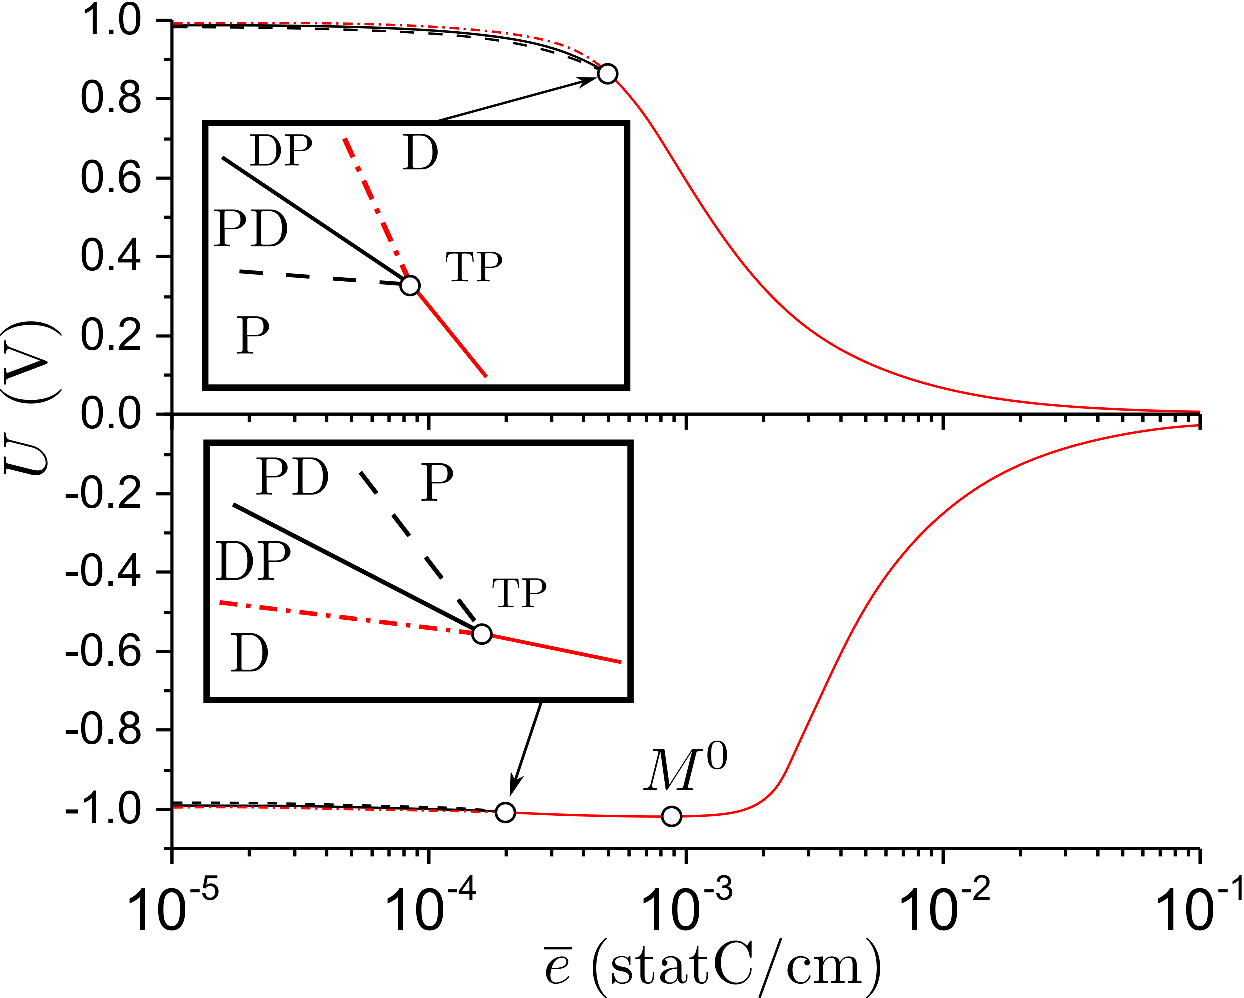
\includegraphics[width=15cm]{Graph7colorB.eps}
	\caption{Фазовая диаграмма.
		Напряжения $U^*$, $U_c$ и $U^{**}$ как функции усреднённого флексоэлектрического коэффициента $\bar{e}$: пунктирная линия -- $U^{**}$, сплошная линия -- $U_c$, штрихпунктирная линия -- $U^{*}$.
		Области стабильности и метастабильности обозначены на вставках.
		Трикритические точки обозначены как TP, другие обозначения совпадают с таковыми на Рис.~\ref{pic-U*U**Uc_otline}.
		Правее трикритической точки TP линии $U^*$, $U_c$ и $U^{**}$ совпадают.}
	\label{pic-U_from_e_pos}
\end{figure}
Интересно отметить, что в случае $U>0$ пороговые напряжения $U^*$, $U_c$ and $U^{**}$ монотонно убывают с ростом $\bar{e}$, то есть в этом случае флексоэлектричество способствует переходу Фредерикса.
Однако эти зависимости оказываются немонотонными для $U < 0$ (точка минимума обозначена как $M^0$).
В случае симметричных границ, то есть, когда $W^{(1)}_\theta = W^{(2)}_\theta$ и $W^{(1)}_\varphi = W^{(2)}_\varphi$, кривые $U^*$, $U_c$ и $U^{**}$ симметричны относительно $U = 0$.
С ростом $\bar{e}$ переход Фредерикса меняет свой род: он оказывается разрывным для небольших $\bar{e}$ и непрерывным для больших $\bar{e}$.
Такая смена рода перехода происходит в трикритической точке TP, окрестность которой схематично показана во вставке на Рис.~\ref{pic-U_from_e_pos}.

\subsubsection{Равновесные ориентационные структуры}

На Рис.~\ref{Fig_profles_sym} представлены равновесные профили $\theta(z)$ и $\phi(z)$, рассчитанные при попарно одинаковых константах сцепления с подложкой (прочие параметры совпадают со стандартным набором).
\begin{figure}%[thb]
	\hspace{0cm}
	\centering
	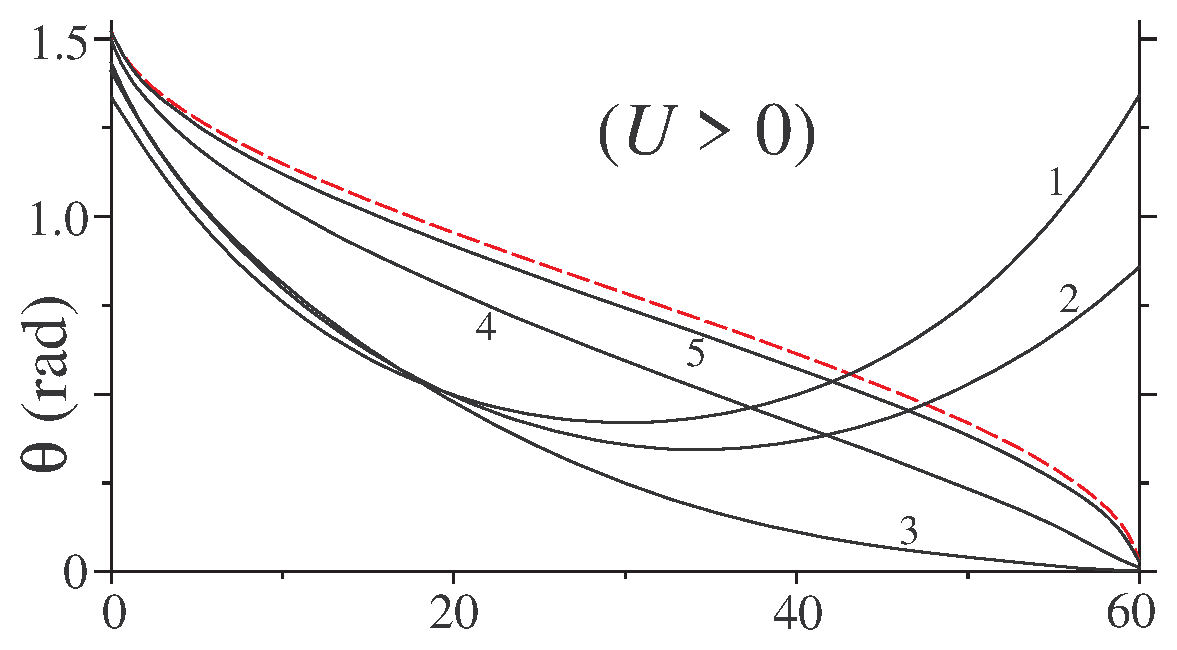
\includegraphics[width=8.5cm]{symm_all_6curvesNoReflect1a.eps}
	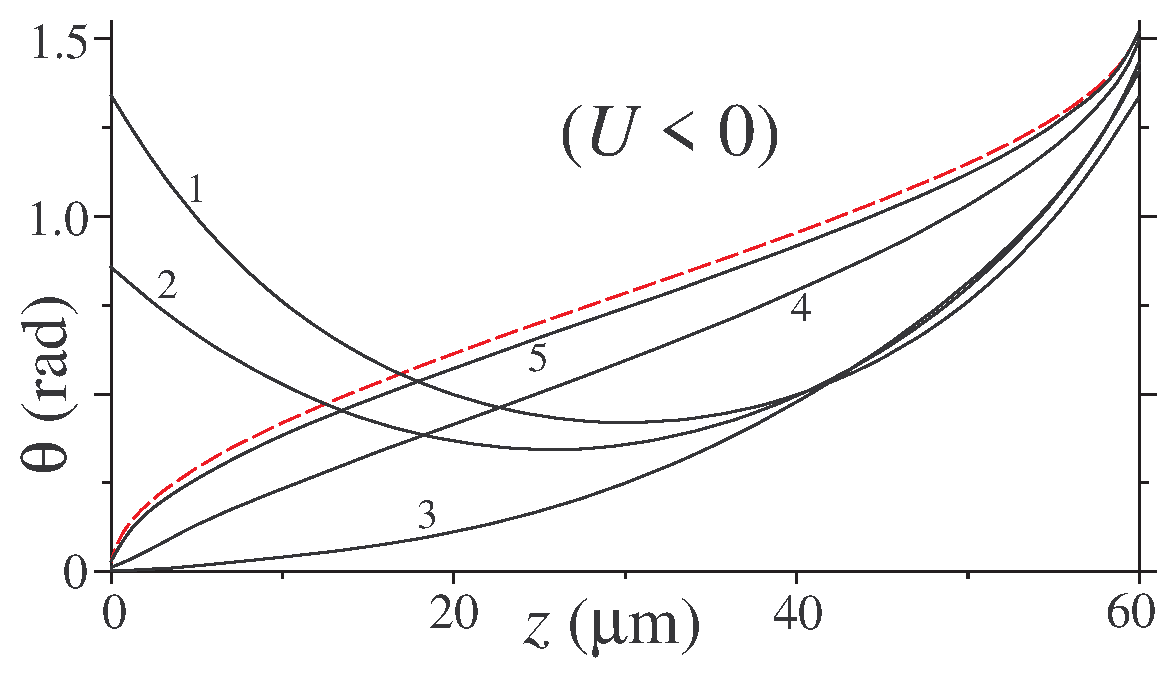
\includegraphics[width=8.5cm]{symm_all_6curvesReflect1.eps}
	\caption{Рассчитанные равновесные профили $\theta(z)$ при $U = \pm 1.2$~В для случая симметричных модулей сцепления с границами: $W_\theta^{(1)}=W_\theta^{(2)}=1.5\times 10^{-3}$~эрг/см$^2$, $W_\phi^{(1)}=W_\phi^{(2)}=1.5\times 10^{-4}$~эрг/см$^2$; остальные параметры стандартные.
	Номера профилей и соответствующие им значения $\bar{e}$ совпадают с таковыми на Рис.~\ref{Fig_profles_nonsym}, кроме графика 2, построенного для $\bar{e} = 5\times 10^{-4}$~Фр/см.
	Красные пунктирные профили рассчитаны по формуле~\eqref{eq_cos2_lin1}.}
	\label{Fig_profles_sym}
\end{figure}
Важно отметить, что именно благодаря флексоэлектричеству профили $\theta(z)$ оказываются асимметричными относительно $z=L/2$.
Это можно пояснить на примере графиков для достаточно больших значений $\bar{e}$.
Из формулы для энергии взаимодействия ХЖК с электрическим полем~\eqref{eq_F_f_final1} видно, что в этом случае основной вклад в свободную энергию даёт слагаемое, содержащее $\bar{e}^2$.
Его можно записать в следующем виде:
\begin{equation}
2\pi S_{\!\bot} \bar{e}^2\int_{0}^{L}\frac{(\sin 2\theta \,\theta'-JJ_1)^2}{{\EE}(\theta)}dz.
\end{equation}
Отметим, что оно принимает минимальное (нулевое) значение, когда $\sin2\theta \, \theta'-JJ_1=0$.
Это интегро-дифференциальное уравнение имеет точное рещение:
\begin{equation}\label{eq_cos2_lin}
\cos^2 \theta(z) =az+b,
\end{equation}
где $a$ и $b$ -- произвольные константы.
При таком $\theta(z)$ член в~\eqref{eq_F_f_final1}, содержащий $\bar{e}^2$, близок к нулю.
Следовательно, главный вклад в $\FF_\mathrm{E}$ даётся вторым слагаемым в~\eqref{eq_F_f_final1}, $S_{\!\bot} \bar{e}U JJ_1\approx S_{\!\bot} \bar{e}U \sin2\theta\, \theta'= -S_{\!\bot} \bar{e}U (\cos^2\theta)'\approx -S_{\!\bot} \bar{e}Ua$.
Для того, чтобы теперь минимизировать  $\FF_\mathrm{E}$, нужно сделать максимальным значение выражения $a\sgn(\bar{e}U)$.
Отметим, что $aL = \cos^2{\theta(L)} - \cos^2{\theta(0)}$, а значит, минимум $\FF_\mathrm{E}$ достигается, когда $\theta(0)\approx\pi/2$, $\theta(L)\approx 0$ для $\bar{e}U>0$ и когда $\theta(0)\approx 0$, $\theta(L)\approx\pi/2$ для $\bar{e}U<0$.
Следовательно, в соответствии с формулами~\eqref{eq_cos2_lin} и \eqref{eq:phi_profile}, при достаточно больших значениях $\bar{e}$ профили углов имеют вид
\begin{equation}\label{eq_cos2_lin1}
\theta(z)\simeq
\begin{cases}
\arccos\sqrt{z/L}, & \bar{e}U>0,\\
\arccos\sqrt{1-z/L}, & \bar{e}U<0,
\end{cases}
\end{equation}
\begin{equation}\label{eq:phi_profile1}
\varphi(z) \simeq
\begin{cases}
\phi_0^{(1)} + \frac{q_0 L}{\zeta} \ln\left( 1 + \zeta\frac{z}{L} \right), & \bar{e}U>0,\\
\phi_0^{(2)} - \frac{q_0 L}{\zeta} \ln\left(1 + \zeta\left(1 - \frac{z}{L}\right)\right), & \bar{e}U<0,
\end{cases}
\end{equation}
где $\zeta = (K_{33} - K_{22})/K_{22}$.
Заметим, что первая формула в~\eqref{eq:phi_profile1} неприменима в окрестности точки $z = L$, а вторая -- в окрестности $z = 0$.
Для того, чтобы корректно описать зависимость $\phi(z)$ в окрестности этих точек, необходимо учитывать в~\eqref{eq_cos2_lin1} малые поправки $\sim 1/\bar{e}$.

Такой же эффект наблюдается и для профилей $\theta(z)$ и $\phi(z)$, рассчитанных для различных $\bar{e}$ и несимметричных констант сцепления с подложкой (в данном случае значения всех материальных параметры совпадают с указанными в предыдущем разделе). Данные профили представлены на Рис.~\ref{Fig_profles_nonsym}.
\begin{figure}%[bth]
%	\hspace{0cm}
	\centering
	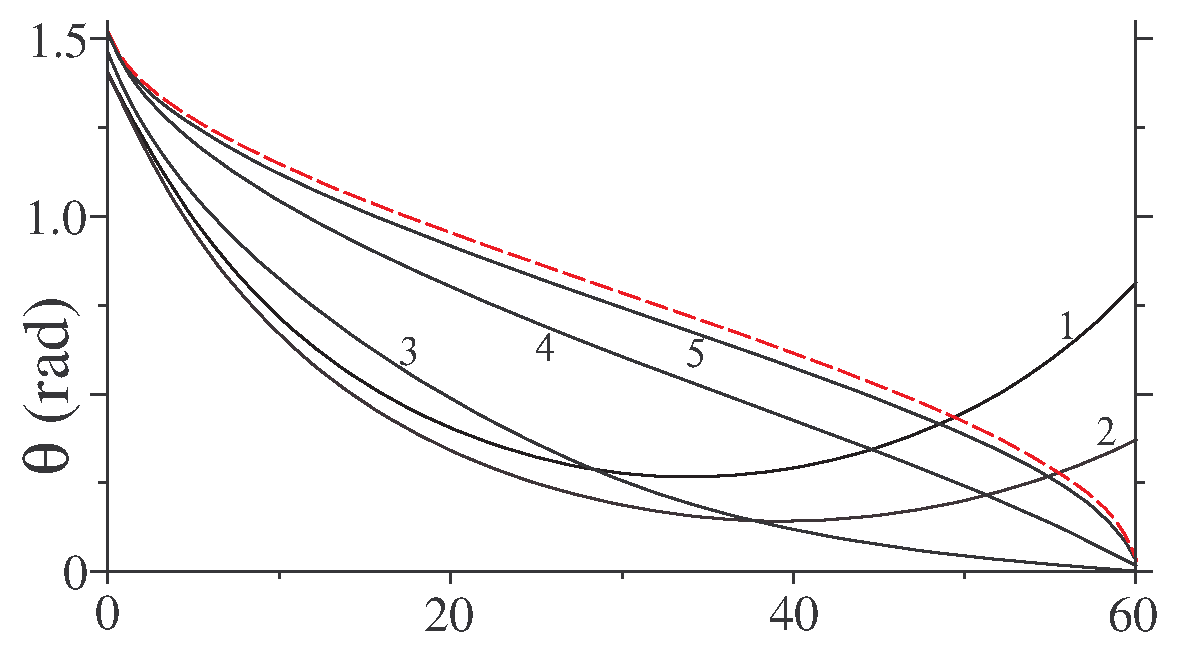
\includegraphics[width=8.5cm]{asymm_theta_6curves1.eps}
	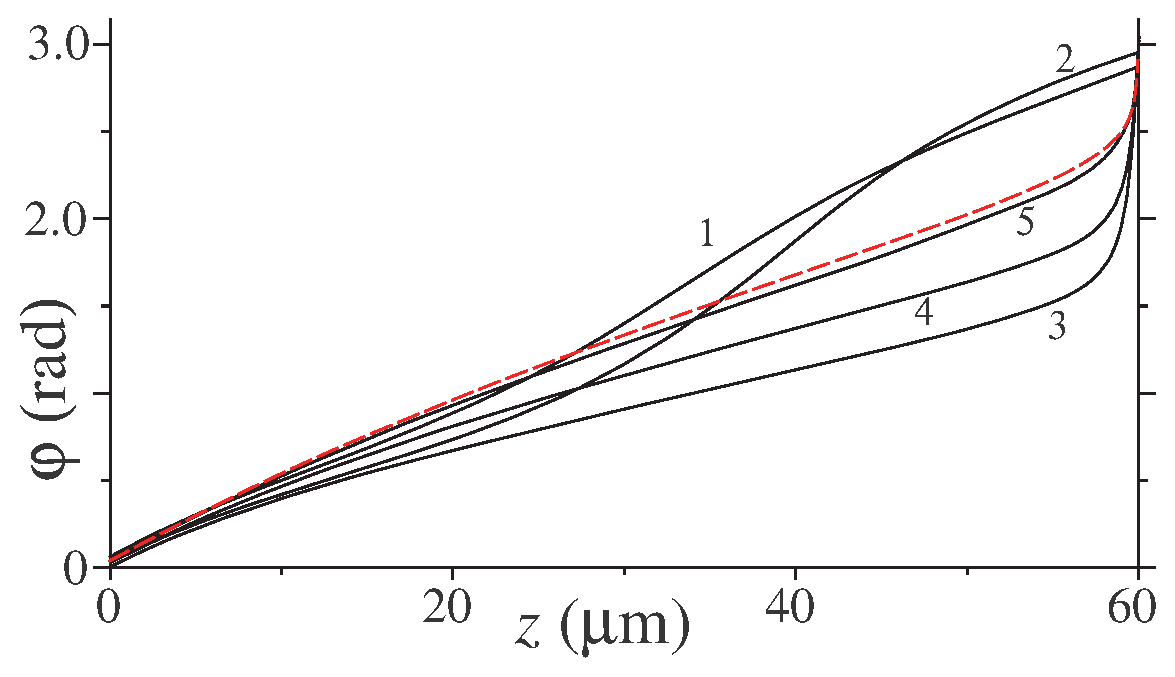
\includegraphics[width=8.5cm]{asymm_phi_6curves1.eps}
	\caption{Равновесные профили $\theta(z)$ и $\phi(z)$, рассчитанные при $U = 1.2$~V. 
		Кривые 1 соответствуют ЖК без флексоэлектричества, $\bar{e}=0$; кривые 2 соответствуют $\bar{e}=10^{-4}$~Фр/см, кривые 3 соответствуют $\bar{e}=10^{-3}$~Фр/см, кривые 4 соответствуют $\bar{e}=3\times 10^{-3}$~Фр/см, а кривые 5 соответствуют $\bar{e}=10^{-2}$~Фр/см. Красные пунктирные линии соответствуют профилям, рассчитанным по формулам~\eqref{eq_cos2_lin1} and~\eqref{eq:phi_profile1}.}
	\label{Fig_profles_nonsym}
\end{figure}
Видно, что и в этом случае при достаточно больших значениях $\bar{e}$ зависимость $\theta(z)$ стремится к рассчитанной выше~\label{eq_cos2_lin1}.

Покажем, как влияет род перехода Фредерикса на ориентационную структуру в ячейке сразу после перехода.
\begin{figure}%[htb]
	\hspace{0cm}
	\centering
	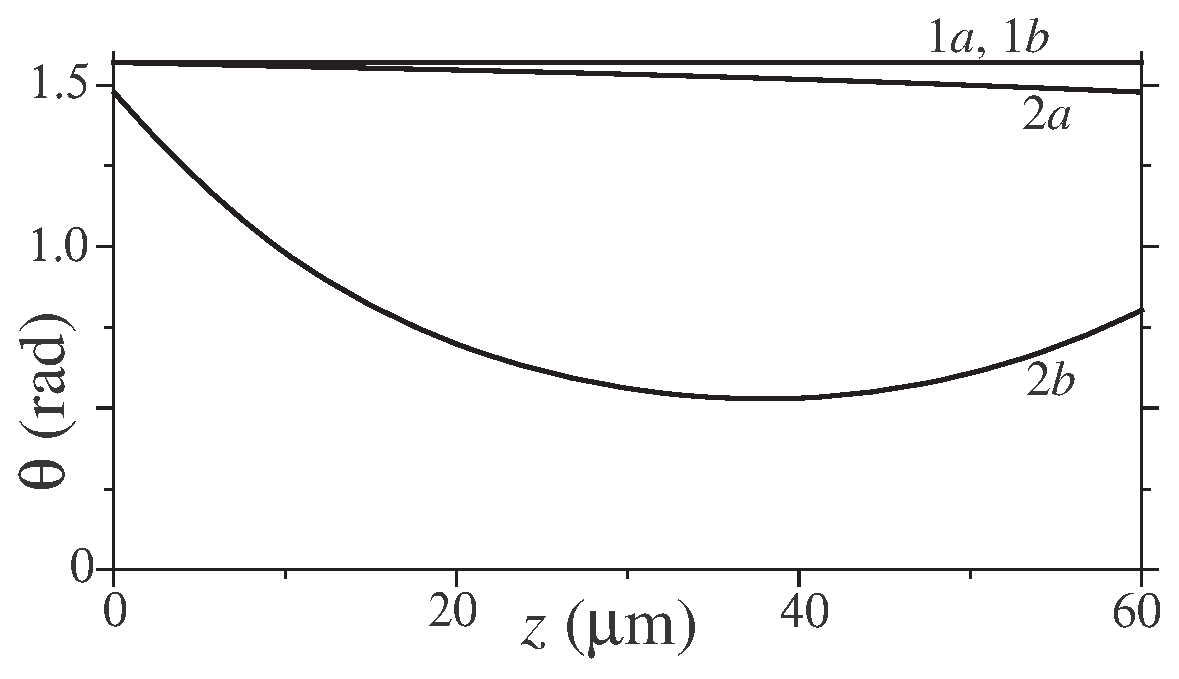
\includegraphics[width=10cm]{1_005Uc_profiles1.eps}
	\caption{Профили $\theta(z)$ для случая непрерывного (a) и разрывного (b) переходов.
		Совпадающие линии профили 1a и 1b соответствуют планарной геликоидальной структуре ($U = 0.999 U_c$), а профили с номером 2 соответствуют искажённым структурам ($U = 1.005 U_c$).
		Для профилей в случае "a": $\bar{e} = 8\times 10^{-4}\text{~Фр/см}<\bar{e}^\text{TP}$, а в случае "b": $\bar{e} = 2\times 10^{-4}\text{~Фр/см}>\bar{e}^\text{TP}$, где $\bar{e}^\mathrm{TP}=5.132\times10^{-4}\text{~Фр/см}$.
		Пороговые значения напряжений составляют: (a) $U_c=0.6926$~В, (b)  $U_c=0.9396$~В.
		Остальные материальные параметры соответствуют таковым на Рис.~\ref{Fig_profles_nonsym}. }
	\label{figCont_Discont_profiles}
\end{figure}
Из Рис.~\ref{pic-U_from_e_pos} можно видеть, что область сосуществования различных ориентационных структур очень узкая при выбранных значениях материальных констант.
%С целью самопроверки
Были рассчитаны профили $\theta(z)$ для двух различных значений $\bar{e}$, больше и меньше $\bar{e}^\text{TP}$ при различных значениях приложенного напряжения.
При напряжении $U < U_c$ структура системы остаётся планарной геликоидальной.
Затем была рассчитана ориентационная структура при напряжении, большем критического $U_c$ на $0.5\%$.
Было обнаружено, что имеется значительное различие между профилями $\theta(z)$ в случае разрывного и непрерывного переходов (Рис.~\ref{figCont_Discont_profiles}).
Следовательно, разрывность перехода значительно меняет ориентационную структуру даже если разница между $U^*$ и $U^{**}$ очень мала.
